%\documentclass[review]{elsarticle}
\documentclass[final,3p,twocolumn]{elsarticle}

\usepackage{lineno,hyperref,amsmath}
%American Mathematical Society mathematical theorems
\usepackage{amsthm}
%American Mathematical Society mathematical symbols
\usepackage{amssymb}
%\usepackage{algorithm}
%\usepackage{algpseudocode}
\usepackage[lined,ruled,commentsnumbered]{algorithm2e}
\usepackage{tikz}
\usetikzlibrary{shapes,arrows,automata,positioning,fit,calc,backgrounds,chains, decorations.pathreplacing}
\usepackage{subfig}
\usepackage{color,soul}
\usepackage[inline]{enumitem}
\usepackage{multirow}

% For nomenclature
\usepackage[intoc]{nomencl}
\makenomenclature

\modulolinenumbers[5]

\journal{Journal of Applied Energy} % 5.746 IF
%\journal{Journal of Energy} % 4.292 IF
%\journal{Journal of Energy Storage} % no IF
%\journal{Journal of Sustainable Energy, Grids and Networks} % no IF

%%%%%%%%%%%%%%%%%%%%%%%
%% Elsevier bibliography styles
%%%%%%%%%%%%%%%%%%%%%%%
%% To change the style, put a % in front of the second line of the current style and
%% remove the % from the second line of the style you would like to use.
%%%%%%%%%%%%%%%%%%%%%%%

%% Numbered
%\bibliographystyle{model1-num-names}

%% Numbered without titles
%\bibliographystyle{model1a-num-names}

%% Harvard
%\bibliographystyle{model2-names.bst}\biboptions{authoryear}

%% Vancouver numbered
%\usepackage{numcompress}\bibliographystyle{model3-num-names}

%% Vancouver name/year
%\usepackage{numcompress}\bibliographystyle{model4-names}\biboptions{authoryear}

%% APA style
%\bibliographystyle{model5-names}\biboptions{authoryear}

%% AMA style
%\usepackage{numcompress}\bibliographystyle{model6-num-names}

%% `Elsevier LaTeX' style
\bibliographystyle{elsarticle-num}
%%%%%%%%%%%%%%%%%%%%%%%

\begin{document}

\begin{frontmatter}

\title{Battery control algorithm for peak load shaving in low-voltage power network with high demand volatility}
%\tnotetext[mytitlenote]{Fully documented templates are available in the elsarticle package on \href{http://www.ctan.org/tex-archive/macros/latex/contrib/elsarticle}{CTAN}.}

%% Group authors per affiliation:
%\author{Elsevier\fnref{myfootnote}}
%\address{Radarweg 29, Amsterdam}
%\fntext[myfootnote]{Since 1880.}

%% or include affiliations in footnotes:
\author[tsbe_address]{Maximilian J. Zangs}
\ead{m.j.zangs@pgr.reading.ac.uk}

\author[tsbe_address]{Timur Yunusov}
\ead{t.yunusov@reading.ac.uk}

\author[sbs_address]{William Holderbaum}
\ead{w.holderbaum@reading.ac.uk}

\author[scs_address]{Ben Potter\corref{correspondingauthor}}
\ead{b.a.potter@reading.ac.uk}
\cortext[correspondingauthor]{Corresponding author}

\address[tsbe_address]{TSBE Centre, J.J. Thomson Building, University of Reading, RG6 6AF, Reading, UK}
\address[sbs_address]{System's Engineering Building, University of Reading, RG6 6AY, Reading, UK}
\address[scs_address]{Chancellor's Building, University of Reading, RG6 6AY, Reading, UK}

\begin{abstract}

Electrification, as a result from ongoing decarbonisation of heat and transport sectors, is increasing the load on UK power distribution networks to a level where service disruptions are expected to occur more frequently.
Distribution Network Operators (DNOs) are anticipating this problem and have trialled deployment of Battery Energy Storage Solutions (BESS) for support of Low-Voltage networks.
This paper presents a dynamic control method that adjusts half-hourly BESS schedules at sub-half-hourly temporal resolution, managing day-ahead half-hourly peaks and sub-half-hourly volatility in demand.
Therefore, the proposed method overcomes drawbacks of traditional controls, which were either too inflexible to cater for today's volatile electricity demand, or which ran the risk of under- or overcharging the energy storage device, if their set-points were badly chosen.
The peak reduction performance of the proposed control method is demonstrated with the use of real sub-half-hourly demand profiles and their corresponding half-hourly load forecasts.
Results indicate additional 18.8\% peak reduction compared to traditional half-hourly BESS operation.

\end{abstract}

\begin{keyword}
Battery Scheduling, Battery Control, Real-Time Correction, Load Forecast
\MSC[2017] 00-01\sep  99-00
\end{keyword}

\end{frontmatter}

\linenumbers

%%%%%%%%%%%%%%%%%%%%%%%%

\printnomenclature%[0.75in]

\section{Overview}
\label{ch2:sec:overview}

%Outages are still very frequent in the UK. 
%According to the UK energy regulator \textit{OFGEM}, on average 45\% of all customers experienced service disruptions in the period 2015-16 \cite{Ofgem2017}.
%Whilst unanticipated outages due to severe winter weather lead to \pounds39 million worth of damages \cite{Ofgem2014}, network upgrades and repairs however contributed the larger amount of customer interruptions and customer minutes lost.
%Such planned outages are intentions to strengthen networks and mitigate system overloads, due to increasing demand for electricity.
%This demand increase is only accelerated since major focus of UK energy policies has been put on transitioning towards a low carbon economy \cite{HMGovernment2009, RoyalAcademyofEngineering2010}.
%Particularly the decarbonisation of heat and transport sectors are two areas of significant strategic focus and Low Carbon Technology (LCT) such as photovoltaic installations, electric vehicles and heat pumps are expected to contribute significantly to this transition.
%
%However, as adaptation of these LCTs increases and they start to penetrate power distribution networks, stress on these networks will continue to increase even further, which may result in additional service disruptions.
%Furthermore, the uptake of LCTs is not expected to progress evenly throughout the entire power network, and instead clusters of early adopters are predicted to form, leading to certain Low-Voltage (LV) networks to exceed their operational constraints even at relatively low national rate of LCT adaption \cite{Poghosyan2014}.
%Traditional network planning approaches to circumvent constraint violations, follow the commonly used practice of aggregating a large number of customers and designing the power delivery network to cater for their largest probable demand, i.e. the After Diversity Maximum Demand (ADMD) method \cite{Richardson2010a}.
%This ADMD method has remained the same for many years and uses historical load analysis and standard growth assumptions that are both no longer valid in this unprecedented LCT uptake scenario \cite{Yunusov2016}.
%To make things worse, LV networks in the UK are generally unmonitored once installed.
%Distribution Network Operators (DNOs) have become aware of this issue and are developing updated planning strategies involving ``smart'' and ``flexible'' electricity grids.
%However, in situ equipment that will become subject to the same adaptation of LCT needs to be managed actively via innovation in the use of existing and new technologies; otherwise both frequency of service disruptions and customer minutes lost will increase alongside the proliferation of LCTs \cite{Ault2008a}.
%
%Two solutions exist, allowing DNOs to support LV network's operation: 
%\begin{enumerate*}
%	\item reinforcement of in situ network assets;
%	\item deployment of network support equipment.
%\end{enumerate*}
%Whilst network reinforcement would certainly address immediate issues of current network capacity constraints, it is also the more expensive and disruptive option.
%More specifically, customer will need to deal with outages during periods of asset upgrades (e.g. transformer upgrade and line re-conductoring after secondary transformers' tap settings have been adjusted).
%Therefore, alternatives to defer or avoid network reinforcements have been sought and assessed \cite{Harrison2007, Zangs2016a, VanderKlauw2016d, Greenwood2017}.
%Most promising alternatives are to install flexible and controllable Distributed Energy Resources (DERs), or more specifically: Battery Energy Storage Solutions (ESMU) \cite{Wade2010}.
%ESMU has not only seen significant advancements in technology, but also received increasing attention in both academic studies and industry trials \cite{Palizban2016}.
%
%Installing ESMU on a strategic location in the LV network brings several advantages to DNOs' control over the network's performance.
%Regulating voltages to stay within statutory operating bands \cite{Yang2014}, shaving peak load to relieve stress from the installed network assets \cite{Bennett2015}, or reducing phase unbalance to increase network efficiency \cite{Wang2015b} are only a few examples of recent research in this field.
%Whilst the questions regarding locating and scaling of ESMU have mostly been addressed, ESMU control can be split into two complementing yet unmarried approaches:
%\begin{enumerate*}
%	\item ``off-line'' control, using load forecasts and ESMU schedules; and
%	\item ``on-line'' control, using Set-Points Control (SPC), Model Predictive Control (MPC) or similar dynamic control methods.
%\end{enumerate*}
%
%Off-line control uses historic data to predict future load patterns, which are used to schedule ESMU operation accordingly.
%Early approaches, e.g. by Oudalov et al. \cite{Oudalov2007}, who used dynamic programming to generate ESMU schedules, had a relatively high forecast error due to the inherent difficulty of predicting future loads, which ultimately limits the ability of given ESMU schedule to i.e. reduce peaks.
%This reason is why recent research either includes uncertainty, like the work by Baker et al. \cite{Baker2017} where uncertainty of wind power was taken into account when scheduling and sizing ESMU, or it frequently re-evaluates ESMU schedules, as done by Wang et.al \cite{Wang2014a}, where ESMU control is adjusted after each decision epoch.
%Despite load forecasts being imperfect, forecasts remain a key component for scheduling ESMU thanks to work like that by Rowe et al. \cite{Rowe2014a}, where a filtering mechanism was proposed for scheduling algorithms to reduce peak load in LV networks in spite of forecast errors.
%Furthermore, most day-ahead forecast only forecast at a temporal resolution down to half-hourly periods.
%As pointed out by Haben et al. \cite{Poghosyan2014, Haben2014}, forecasts at half-hourly resolution yield the best compromise between high accuracy and high temporal resolution, which is why they have become the standard for generating ESMU operating schedules.
%Nonetheless, sub-half-hourly load volatility imposes the biggest stress on the network and cannot be addressed when using this kind of half-hourly forecast, which is why on-line control has been considered as an alternative to off-line control.
%
%One flavour of on-line control is the Set-Point Control (SPC), which is a robust technique that can immediately respond to network changes.
%Since this kind of control runs the risk of reaching shortage or surplus of ESMU stored energy, modifications like hysteresis control \cite{Gybel2012} and ramp-rate control \cite{Such2012} were proposed.
%However, this kind of on-line control is less effective in addressing daily demand peaks, since pure SPC can only react to current network demand and does not respond to general trends or upcoming load events.
%To address these shortcomings SPC has been extended, using short-term load predictions by implementing Model Predictive Control (MPC).
%Some MPC examples include Auto-Regressive (AR) models \cite{Li2009, Nie2011}, fuzzy logic models \cite{Sannomiya2001, Chen2013a}, genetic algorithms \cite{Xia2015a, Liu2015} or Artificial Neural Networks (ANN) \cite{Kalogirou2014, Quan2014, Lee2014, Pezeshki2014, Vaz2016, Reihani2016, Xiao2017}.
%Implementing increasingly complex MPC to support on-line control is therefore a strong research trend, however the computational burden to deliver real-time solutions makes implementation of such systems not yet feasible.

\nomenclature[G]{SPC}{Set-Point Control}
\nomenclature[G]{MPC}{Mode-Predict Control}
\nomenclature[G]{PID}{Proportional Integrating Derivative (control)}


In the preceding chapter an Energy Storage Management Unit (ESMU) is used to improve network operation.
This improvement is achieved by optimally adjusting the device's scheduled three-phase powers.
Any improvement is indicated by reduction of cost functions, which are tied to key network parameters.
By focusing on different costs and repetitively optimising and simulating the ESMU powers, shows the extend by which the device can improve the network's operation.
However, this improvement is limited by the constraint of having to obey the underlying half-hourly ESMU schedule, despite applying adjustments at a sub-half-hourly level.

In the following chapter, this limiting constraint is lifted, and the corresponding sub-half-hourly ESMU schedule adjustment method is proposed.
This method unifies the benefits from sub-half-hourly demand measurements and half-hourly demand forecasts.
Unlike previous work in the field, the proposed approach reverses the traditional control paradigm to compensate for schedule inaccuracies.
To reiterate, these traditional approaches implemented on-line control mechanisms, e.g. Set-Point Control (SPC), in combination with prediction models in order to adjust and prepare ESMU for future load trends.
In this presented work however, instead of supporting on-line control with real-time load predictions, forecast driven schedules are adjusted using on-line measurements.
This is achieved by first scheduling ESMU operation at half-hourly resolution, i.e. by following a ``peak-shaving'' and ``valley-filling'' behaviour which has been explained in Chapter \ref{ch1}, and then modifying this schedule using MPC.
In this case, MPC is comprised of of a lightweight AR model to assure real-time deployability.
These two control signals are unified using two Proportional Integral Derivative (PID) compensators that are tuned to assure system robustness, regardless of the forecast's erroneousness.
All ESMU schedules are generated under the constraints of a realistic ESMU model, and all demand measurements and corresponding forecasts used in this work are based on real data, provided by the project partner and DNO: \textit{Scottish and Southern Energy Networks} (SSEN).
Results are generated from this realistic (i.e. provided) network load with corresponding load forecasts, and cases are compared against the original and a baseline load case (i.e. traditional off-line control).
It is shown that, even under these imperfect forecast conditions, the proposed schedule adjustment method can successfully reduce sub-half-hourly peaks.
In fact, whilst the probability distribution of the baseline case sat around an average of 1.78kW peak reduction, the proposed method increased the reduction to 5.24kW.
Since this proposed control method is the natural extension of our previous work in \cite{Zangs2016}, it is hereon referred to as ``dynamic control''.

The chapter is organised as follows:
In Section \ref{ch2:sec:system-explanation}, all constituent system components including ESMU model, forecast acquisition and ESMU schedule generation are explained.
%Cost functions to generate optimised half-hourly ESMU schedules are formulated, containing well established parameters like the Peak-to-Average Ratio (PAR) or ``Min-Max'' difference, which have been widely used in DER scheduling and operation \cite{Liu2014, Deng2015, Bayram2015, Zangs2016a}.
Section \ref{ch2:sec:control-of-ESMU} presents the dynamic control, including the dual PID setup and MPC.
Section \ref{ch2:sec:case-studies} outlines the different case studies that were used to compare the performance of the dynamic control.
In Section \ref{ch2:sec:results}, all results from these case studies are presented and discussed.
Finally, conclusion and the future work are described in Section \ref{ch2:sec:summary}.












\section{System Explanation}
\label{ch2:sec:system-explanation}

\begin{figure}[htb]\centering
% Define some block styles
\tikzstyle{box} = [%
	draw,%
	rectangle,%
	%fill=green!20,%
	minimum height=3em,%
	minimum width=5em,%
]
\subfloat[]{%
	\begin{tikzpicture}[node distance=1.5cm, shorten >= 1pt, >=stealth', auto, scale=0.8, transform shape]
		% Define nodes
	    \path (0,0)
	    node [box, fill=blue!20](data) {Data}
	    node [box, fill=blue!20, below of=data](forecast) {Forecast}
	    node [box, fill=blue!20, below of=forecast](schedule) {Schedule}
	    node [box, below of=schedule](battery) {Battery}
	    node [box, below of=battery](network) {Network};
		% Draw lines
		\draw [->] (data) to (forecast);
		\draw [->] (forecast) to (schedule);
		\draw [->] (schedule) to (battery);
		\draw [->] (battery) to (network);
	\end{tikzpicture}%
	\label{ch2:subfig:traditional-forecast-based-system}%
}
\hspace{10mm}
\subfloat[]{
	\begin{tikzpicture}[node distance=1.5cm, shorten >= 1pt, >=stealth', auto, scale=0.8, transform shape]
		% Define nodes
	    \path
	    (0,0) 
	   	node [box, fill=green!20, below of=schedule, xshift=-14.5mm](controller) {Controller}
		node [box, fill=green!20, below of=controller](mpc) {MCP}
	    node [box, right of=controller, xshift=15mm](battery) {Battery}
	    node [box, below of=battery](network) {Network};;
		% Draw lines
		\draw [->] (network) to (mpc);
		\draw [->] (mpc) to (controller);
		\draw [->] (controller) to (battery);
		\draw [->] (battery) to (network);
	\end{tikzpicture}%
	\label{ch2:subfig:traditional-on-line-system}%
}
\hspace{10mm}
\subfloat[]{%
	\begin{tikzpicture}[node distance=1.5cm, shorten >= 1pt, >=stealth', auto, scale=0.8, transform shape]
		% Define nodes
	    \path
	    (0,0)
	    node [box, fill=blue!20](data) {Data}
	    node [box, fill=blue!20, below of=data](forecast) {Forecast}
	    node [box, fill=blue!20, below of=forecast](schedule) {Schedule}
	    node [box, below of=schedule](battery) {Battery}
	    node [box, below of=battery](network) {Network}
	   	node [box, fill=green!20, left of=battery, xshift=-14.5mm](controller) {Controller}
		node [box, fill=green!20, below of=controller](mpc) {MCP};
		% Draw lines
		\draw [->] (data) to (forecast);
		\draw [->] (forecast) to (schedule);
		\draw [->, bend right] (schedule.180) to (controller.90);
		\draw [->] (network) to (mpc);
		\draw [->] (mpc) to (controller);
		\draw [->] (controller) to (battery);
		\draw [->] (battery) to (network);
	\end{tikzpicture}%
	\label{ch2:subfig:proposed-hybrid-system}%
}

\caption{Combination of traditional forecast driven BESS control (Subfig. \ref{ch2:subfig:traditional-forecast-based-system}) and traditional on-line system (Subfig. \ref{ch2:subfig:traditional-on-line-system}) results in the proposed hybrid system (Subfig. \ref{ch2:subfig:proposed-hybrid-system}).}
\label{ch2:fig:system-diagram}
\end{figure}


The presented work is part of the \textit{New Thames Valley Vision} (NTVV) research project, and was conducted in collaboration with the British DNO \textit{Scottish and Southern Energy Networks} (SSEN) \cite{NTVV2016}.
From the findings of this research project, the diagram in Figure \ref{ch2:fig:system-diagram} was generated, showing two well established ESMU control approaches and the proposed dynamic control approach.
This figure includes all constituent systems that were used during the ESMU street-level deployment.
The two traditional systems are off-line and on-line ESMU control, which are shown in Figure \ref{ch2:subfig:traditional-forecast-based-system} and \ref{ch2:subfig:traditional-on-line-system}, respectively.
Alongside these two control approaches is the proposed dynamic control system, as shown in Figure \ref{ch2:subfig:proposed-dynamic-control-system}.
This control approach entails the benefits from both the traditional half-hourly forecast driven and the sub-half-hourly ESMU control system, and can therefore be seen as the hybrid of the two traditional systems.
Unlike previous work however, this hybrid system does not use Set-Point Control (SPC), which is aided by a MPC to compensate for trends in the load profile.
Instead, it operates by executing a predetermined half-hourly ESMU schedule with sub-half-hourly adjustments.
Those adjustments are based on MPC-guided instructions, and details about this dynamic control are outlined in Section \ref{ch2:sec:control-of-esmu}.

In this section however the battery model, which is used in this work, is explained first.
Also the load data acquisition, forecasting and ESMU schedule generation are outlined, where scheduling is performed in accordance to the ESMU model's constraints.

\subsection{ESMU model}

\nomenclature[J]{$C_{bat}$}{Battery capacity in kWh, where $C_{bat} \in \mathbb{Z}^{>0}$}
\nomenclature[J]{$C_{f}$}{Charge factor or ``C-factor'' of the battery, where $C_{f} \in \mathbb{Z}^{>0}$}
\nomenclature[J]{$\mu$}{Self-discharge losses of battery, where $\mu \in (0, 1]$}
\nomenclature[J]{$P_{bat}$}{ESMU power electronic rating, where $P_{bat} \in \mathbb{Z}^{>0}$}
\nomenclature[J]{$\eta$}{Round-trip efficiency of power electronics, where $\eta \in (0, 1]$}
\nomenclature[J]{$t$}{Discrete sample of time, where $t \in \{0, \Delta t, \dots, T\Delta t\}$}
\nomenclature[J]{$T$}{Number of samples during the entire simulation, where $T \in \mathbb{Z}_{>0}$}
\nomenclature[J]{$\Delta t$}{Sub-half-hourly sample period, where $\Delta t \in \mathbb{Z}^{>0}$}
\nomenclature[J]{$SOC(t)$}{Scheduled state of charge at sample $t$}
\nomenclature[J]{$p(t)$}{ESMU power at time $t$, where $\textbf{p} = (p(t))$ and $p(t) \in \mathbb{Z}$}
\nomenclature[J]{$\textbf{p}$}{ESMU power vector, where $\textbf{p} = (p(t))$}
\nomenclature[J]{$p_{bat}(t)$}{Battery power at time $t$, which is derived form $p(t)$, where $\textbf{p}_{bat} = (p_{bat}(t))$ and $p(t) \in \mathbb{Z}$}
\nomenclature[J]{$\textbf{p}_{bat}$}{Battery power vector, where $\textbf{p}_{bat} = (p_{bat}(t))$}

The ESMU model is based on the physical system that was deployed by SSEN during the NTVV project.
Since this model is the same model as the one used in the preceding chapter, which has been explained in detail in Section \ref{ch1:subsec:battery-model}, only the model's final equation (as well as all used parameters) are detailed, hence foregoing the re-deriving of the same battery storage model.
This ESMU model equation is as follows:

%Therefore, the model is designed to accurately capture the physical limitations of the device, which includes a limited capacity of the battery pack, $C_{bat}$, and a corresponding charge and discharge factor (i.e. the ``C-factor''), $C_{f}$, to also limit the maximum charge and discharge rate\footnote[1]{Nominal charge and discharge powers are calculated from the ``C-factor'' and the capacity of the battery. For example, a 12.5kWh battery with a C-factor of 1.6(h$^{-1}$) would have a maximum dis/charge rate of 20kW ($=12.5 \cdot 1.6$).}.
%Furthermore, the power electronics unit that regulates the three-phase power flow into and out of the ESMU is limited by its power ratings, $P_{bat}$, which must not be exceeded.
%Corresponding conversion losses within the power electronics unit lead to a limited ESMU round-trip efficiency, $\eta$, where $\eta \in (0, 1]$.
%Self-discharge losses inside the battery pack are also included as the ratio $\mu$, where $\mu \in (0, 1]$.
%This ratio expresses how much energy is lost over time, due to the battery's imperfect means of storing energy.
%
%The dynamics of ESMU are modelled over discrete time, $t$ where $t \in \mathbb{Z}_{\geq0}$, by simulating the transition from one State of Charge (SOC) to the next.
%A finite sampling period between each simulation's time-step is defined and notated as $\Delta t$, and this sample period represents the highest temporal resolution used in the context of this work, i.e. sub-half-hourly resolution.
%Change in State of Charge, i.e. $\delta SOC(t)$, can then be defined as the difference between the current State of Charge, $SOC(t)$, and the subsequent State of Charge, $SOC(t+\Delta t)$.
%When combining this definition with the self-discharge loss, the following SOC equation can be formulated:
%
%\begin{equation}
	SOC(t+\Delta t) := \eta(SOC(t) + \delta SOC(t))
	\label{ch2:equ:soc-equation}
\end{equation}
%
%Hence, $\delta SOC(t)$ is the result of charging or discharging the battery by consuming or releasing energy.
%The amount of energy that flows into or out of the ESMU is equal to the active power, $p(t)$, that is applied over the sampling period $\Delta t$.
%Yet $\delta SOC(t)$ is not equal to this consumed energy, due to the imperfect round-trip efficiency.
%In order to act like a load in the LV network, positive power is associated to charging and negative power is associated to discharging the ESMU.
%Therefore, the sign of the ESMU power indicates the direction of the flowing energy, and based upon this direction of energy flow, the true amount of stored charge can be calculated by using the aforementioned round-trip efficiency, $\mu$.
%In order to correctly inject or absorb power into or from the network, ESMU power is given and battery power, $p_{bat}(t)$, is derived and defined as follows:
%
%\begin{equation}
	p_\text{bat}(t) =
	\begin{cases}
		\mu p(t) &\text{if } p(t) \geq 0\\
		\frac{1}{\mu}p(t) &\text{otherwise}
	\end{cases}
	\forall t
	\label{ch2:equ:battery-power}
\end{equation}
%
%As power electronics approach ideal performance, $\mu$ tends towards one, however a value of $0.95$ is chosen for the model to coincide with the technical specifications of the deployed ESMU units.
%Knowing both the power at street- and at the battery-level, the amount of energy injected into the battery during $\Delta t$ can be determined:
%
%\begin{equation}
	\delta SOC(t) = \frac{\tau}{C_{battery}}p_{battery}(t)
	\label{ch2:equ:soc-equation-from-battery-power}
\end{equation}
%
%Combining Equation \ref{ch2:equ:soc-equation}, \ref{ch2:equ:battery-power} and \ref{ch2:equ:soc-equation-from-battery-power} and solving for $SOC(t+\Delta t)$, yields the following battery model equation:

\begin{equation}
	SOC(t+\tau) =
	\begin{cases}
		\mu \left(SOC(t) + \eta \frac{\tau}{C_{battery}}p(t)\right) &\text{if } p(t) \geq 0\\
		\mu \left(SOC(t) + \frac{1}{\eta} \frac{\tau}{C_{battery}}p(t)\right) &\text{otherwise}
	\end{cases}
	\forall t
	\label{ch2:equ:battery-model-equation}
\end{equation}

Here, the next State of Charge, $SOC(t+\Delta t)$, is computed from the current State of Charge, $SOC(t)$, and the battery power, $p(t)$.
This is done by calculating the change in SOC as the currently added energy $\Delta t p(t)$, divided by the battery capacity $C_\text{bat}$.
Dynamics of the model also take into account the energy conversion efficiency, $\eta$, and the self-discharge factor, $\mu$.

For the purpose of the simulation, it is assumed that the battery is initially charged up to 50\%.
Hence, the initial conditions of this model are defined as $SOC(0) = 0.5$, which makes the model valid for a time span of $t \geq 0$, where $t \in \mathbb{Z}_{\geq0}$.

\subsection{Load data and ESMU scheduling}

\nomenclature[J]{$k(t)$}{Sampling time conversion function, linking sub-half hourly samples $t$ at sampling period $\Delta r$ to half-hourly period $30 \Delta t$}

Having established the ESMU model, the procedure to generate a corresponding schedule is explained in this section.
This procedure follows the same practice as outlined in the previous chapter, in Section \ref{ch1:subsec:esmu-scheduling}, where an ESMU schedule is generated at half-hourly temporal resolution.
Therefore, the same synchronisation function, $k(t)$, is used that links the native sampling period of $\Delta t$, to the schedule's half-hourly period.
Since the sub-half-hourly operation was at a minutely period, and the generated schedule is at half-hourly period, this fixed conversion function is defined as:

\begin{equation}
	k(t) := \left\lfloor\frac{t-1}{30\Delta t}\right\rfloor+1
	\label{ch2:equ:sample-conversion-function}
\end{equation}

Having established a means of synchronising the two sampling periods, the wanted behaviour of the ESMU schedule is defined next.
For simplicity linear forwarding was chosen, which means that the power assigned at e.g. $t=1$ remains constant over the scheduling period of $30\Delta t$, until $t=31$.
With this assumption, the ESMU's SOC can be calculated for each $t$ despite the scheduled power profile only having been defined for every 30$^\text{th}$ $t$.
Furthermore, with this second assumption, not only every sub-half-hourly ESMU power can be derived from its half-hourly schedule, but it also enables the calculation of every SOC, i.e. $SOC(t)$ is well defined.

\nomenclature[J]{$p_\text{for}(k(t))$}{Half-hourly load forecast that is used for computing the ESMU schedule, where $p_\text{for}(k(t))\in\mathbb{Z}$}
\nomenclature[J]{$\textbf{p}_\text{for}$}{Half-hourly load forecast vector that is used for computing the ESMU schedule, where $\textbf{p}_\text{for} = (p_\text{for}(k(t)))$}
\nomenclature[J]{$p_\text{sch}(k(t))$}{Half-hourly schedule that is generated from the load forecast, where $p_\text{sch}(k(t))\in\mathbb{Z}$}
\nomenclature[J]{$\textbf{p}_\text{sch}$}{Half-hourly schedule vector that is generated from the load forecast, where $\textbf{p}_\text{sch} = (p_\text{sch}(k(t)))$}

For the generation of the ESMU schedule a load forecast, $\textbf{p}_\text{for}$, was required; here $\textbf{p}_\text{for} = (p_\text{for}(k(t)))$.
This forecast, similar to the ESMU schedule, is also at half-hourly temporal resolution and is provided by SSEN as part of the NTVV research project.
The task at hand is to find a half-hourly ESMU schedule, $\textbf{p}_\text{sch}$, where $\textbf{p}_\text{sch} = (p_\text{sch}(k(t)))$, that improves the shape of the underlying forecast, e.g. by reducing load peaks.
In order to generate this optimised ESMU schedule, a metric quantifying improvements had to be defined first.
The only remaining problem is to find a half-hourly schedule, $\textbf{p}_\text{sch}$, which is done through by minimising several cost-functions.

In this work, three cost-functions are used that quantify the network improvements, yielded by $\textbf{p}_\text{sch}$.
These costs entailed the Peak-to-Average Ratio (PAR), the difference between the resulting power profile's maximum and minimum (MMD) load, and the magnitude of all power transients (TRA) \cite{Mohsenian-Rad2010, Mostafa2016}.
Before explaining each of these three cost functions however, a notation simplifying power as, $\textbf{p}$, is introduced:

\begin{equation}
\begin{split}
	p(t) = p_{for}(k(t)) + p_{sch}(k(t))\\
	\text{ where } \textbf{p} = (p(t))
\end{split}
\label{ch2:equ:notation-simplification}
\end{equation}

Within this section, the vector $\textbf{p}$ represents the power profile as it would be measured at the substation when both forecast, $p_\text{for}(t)$, and scheduled, $p_\text{sch}(t)$, power were applied.
The first cost function, addressing the minimisation of PAR, is defined as follows:

\nomenclature[J]{$\zeta_\text{PAR}(\textbf{p})$}{Cost of a power profile $\textbf{p}$, based on Peak-to-Average Ratio (PAR), where $\zeta_\text{PAR}(\textbf{p}) \in \mathbb{R}_{\geq0}$}

\begin{equation}
	\zeta_{PAR}(\textbf{p}) := \frac{\max_t|\textbf{p}|}{\overline{\textbf{p}}} - 1%\frac{\max_t|p(k(t))|}{\frac{1}{T}\sum_{t=1}^Tp(k(t))} - 1
	\label{ch2:equ:cost-par}
\end{equation}

\nomenclature[J]{$T_\text{sch}$}{Length of scheduling horizon, where $T_\text{sch} \in \mathbb{Z}_{>0}$ and $T \geq T_\text{sch}$}

Here, $\overline{\textbf{p}}$ represents the mean power, i.e. $\overline{\textbf{p}} = \frac{\Delta t}{T_\text{sch}}\sum_{t=1}^{T_\text{sch}}p(t)$ and $\overline{\textbf{p}} \in \mathbb{R}$, where $T_\text{sch}$ is the length of the scheduling horizon in regards to the sampling period $\Delta t$.
From this cost, a perfect power profile would yield a PAR cost of zero, if the profile is a perfectly flat.
However, due to limited battery capacity, achieving such a cost of zero is unlikely.
The second cost function represents the difference between minimum and maximum power of $\textbf{p}$:

\nomenclature[J]{$\zeta_\text{MMD}(\textbf{p})$}{Cost of a power profile $\textbf{p}$, based on the difference between minimum and maximum power, where $\zeta_\text{MMD}(\textbf{p}) \in \mathbb{R}_{\geq0}$}

\begin{equation}
	\zeta_\text{MMD}(\textbf{p}) := (\max_t(\textbf{p}) - \min_t(\textbf{p}))^2
	\label{ch2:equ:cost-min-max}
\end{equation}

Similar to the PAR, this cost also reduces to zero when the resulting power profile is a perfectly flat line.
Unlike the PAR, this cost does not incentivise an increase of mean power.
Minimising PAR by itself may result in unnecessary and potentially damaging battery cycling, when trying to elevate the power profile's mean, yet this is avoided when $\zeta_\text{MMD}$ is included alongside $\zeta_\text{PAR}$.
However, $\zeta_\text{PAR}$ and $\zeta_\text{MMD}$ only impact the fringes of the resulting half-hourly power profile.
The final cost therefore addresses the interim power volatility by aiming to minimise the largest possible power transient:

\nomenclature[J]{$\zeta_\text{TRA}(\textbf{p})$}{Cost of a power profile $\textbf{p}$, based on largest power transient, where $\zeta_\text{TRA}(\textbf{p}) \in \mathbb{R}_{\geq0}$}

\begin{equation}
	\zeta_\text{TRA}(\textbf{p}) := \max_{t}(p(t+\Delta t)-p(t))^2
	\label{ch2:equ:cost-tra}
\end{equation}

Minimising this final cost has a smoothening effect on the improved half-hourly power profile, since a profile with no transients is by definition a flat smooth profile.
All three cost functions are summaries into a single global cost function, where only the half-hourly ESMU schedule, $\textbf{p}_\text{sch}$, is used as an input and the forecast, $\textbf{p}_\text{for}$, is kept as constant:

\nomenclature[J]{$\zeta(\textbf{p})$}{Global cost for a given power profile $\textbf{p}$}
\begin{equation}
\begin{split}
	\zeta(\textbf{p}_{sch}) := &\zeta_\text{PAR}(\textbf{p}_{sch}+	\textbf{p}_{for})\\
	&+ \zeta_\text{MM}(\textbf{p}_{sch}+\textbf{p}_{for})\\
	&+ \zeta_\text{TRA}(\textbf{p}_{sch}+\textbf{p}_{for})
\end{split}
\label{ch2:equ:cost-global}
\end{equation}

Subject to ESMU constraints, this global cost function is minimised using a standard solver (i.e. Sequential Quadratic Programming - SQP) to yield a ESMU schedule that is optimised for the given forecast:

\begin{equation}
	\min_{\textbf{p}_{sch}}\zeta(\textbf{p}_{sch})
	\text{ s.t. }
	\begin{cases}
		SOC_{tol} \leq SOC(t)\\
		SOC(t) \leq 1-SOC_{tol}\\
		|p_{bat}(t)| \leq C_{bat} \times C_{f}
	\end{cases}
\label{ch2:equ:cost-minimisation}
\end{equation}

In order to limit the control's flexibility, a State Of Charge tolerance, $SOC_{tol}$, is included in this minimisation problem.
$SOC_{tol}$ defines the maximum allowed deviation from the computed SOC profile without hitting operational limits, i.e. SOC of one or zero, and may take values in the form of $SOC_{tol} \in [0, 0.5]$, where 0 implies no tolerance and 0.5 implies complete flexibility.
For the work at hand, a value of 0.1 was chosen.

\begin{figure}\centering
	\subfloat[]{%
		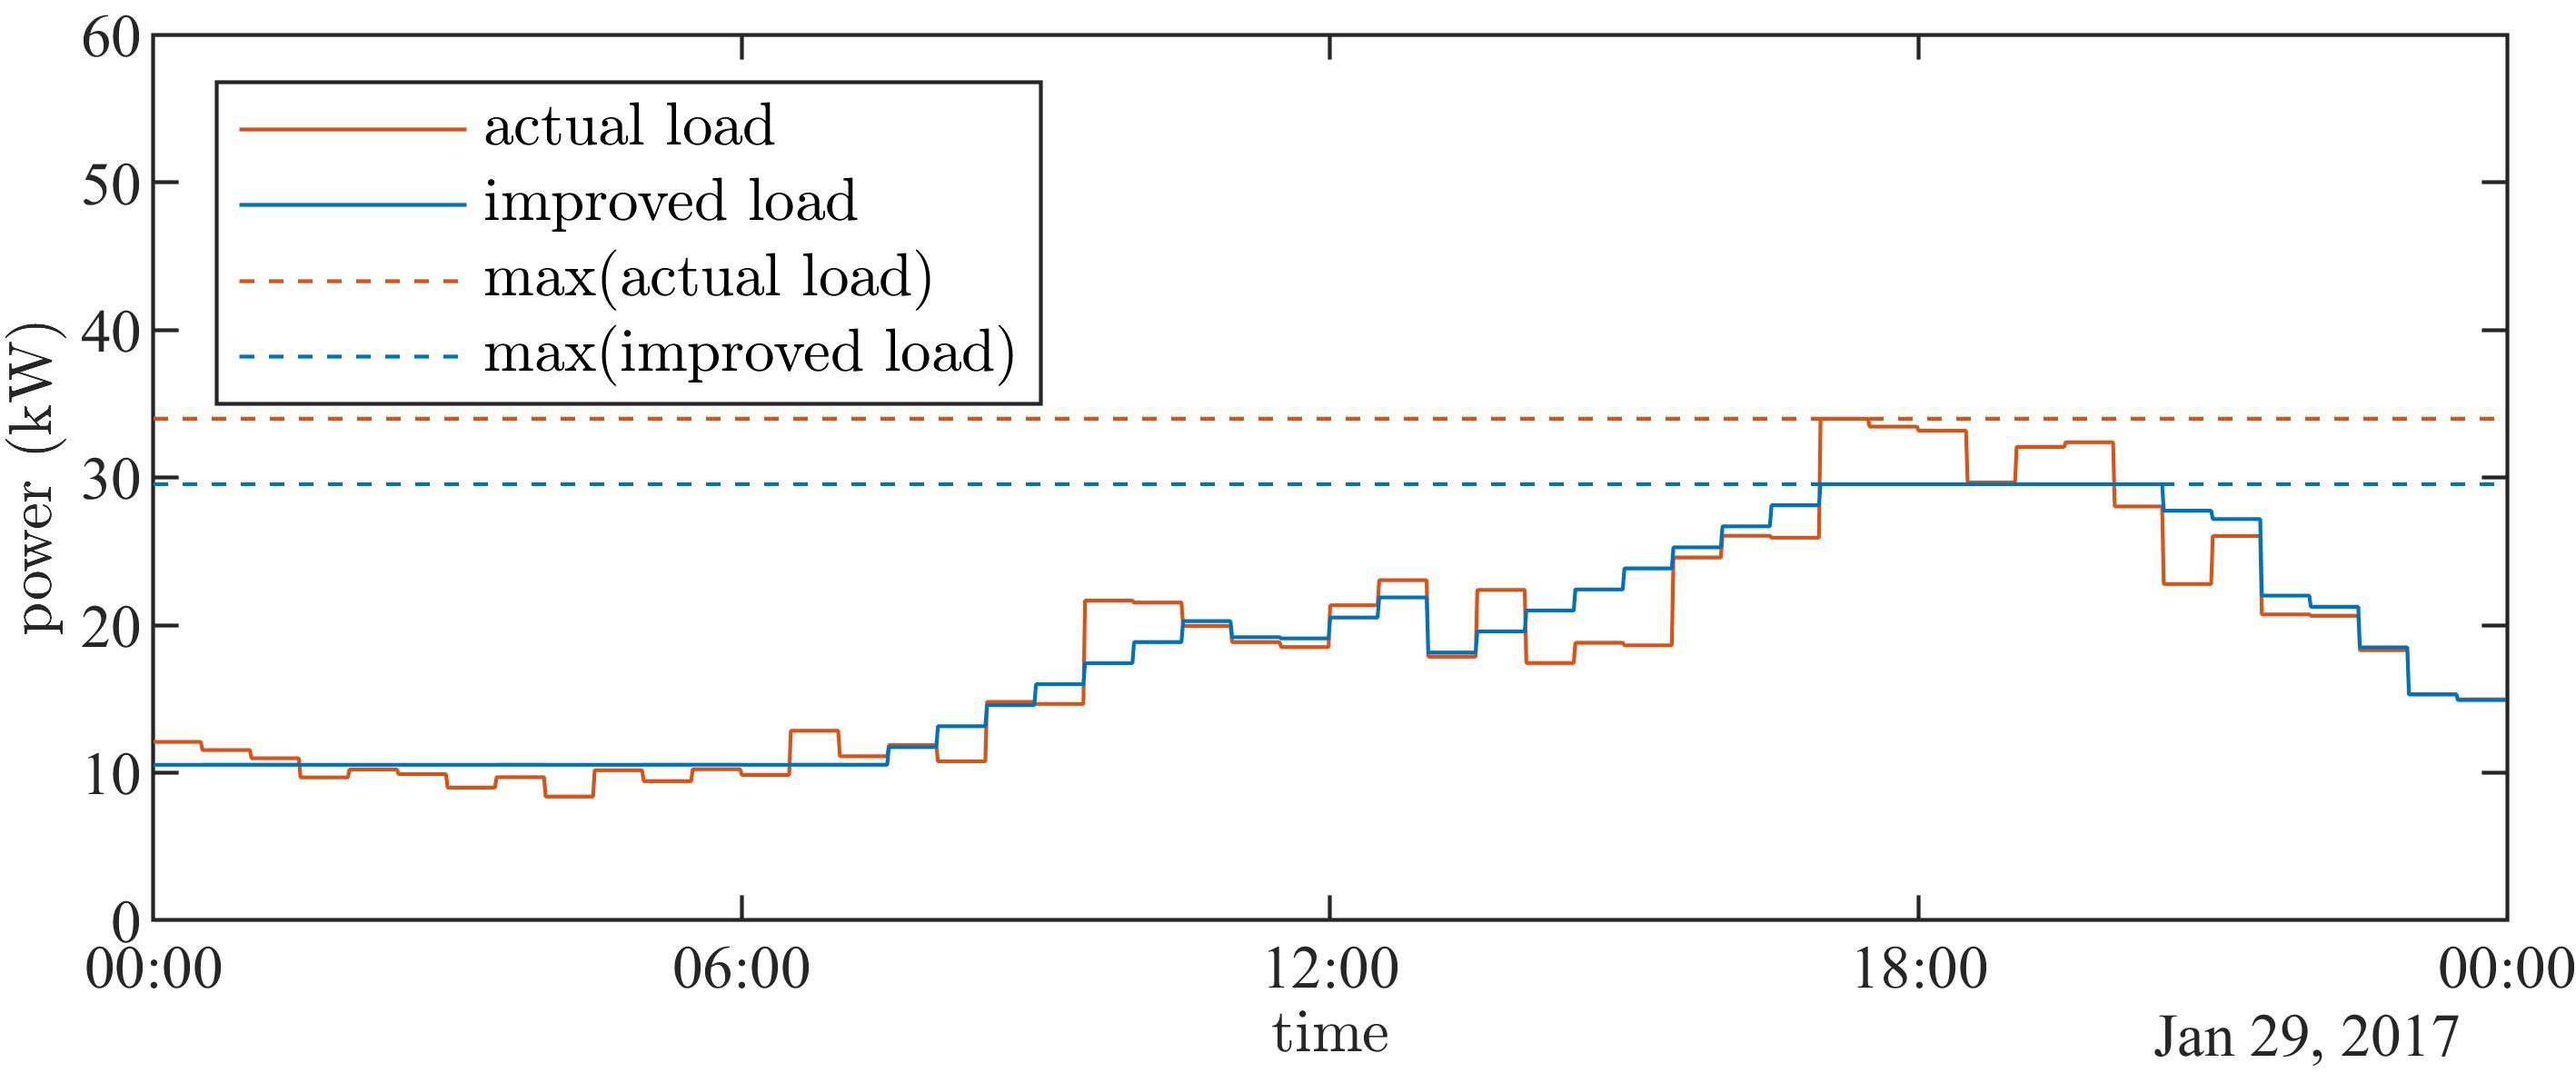
\includegraphics{_chapter2/fig/day-forecasted}
		\label{ch2:subfig:day-forecasted}
	}\\
	\subfloat[]{%
		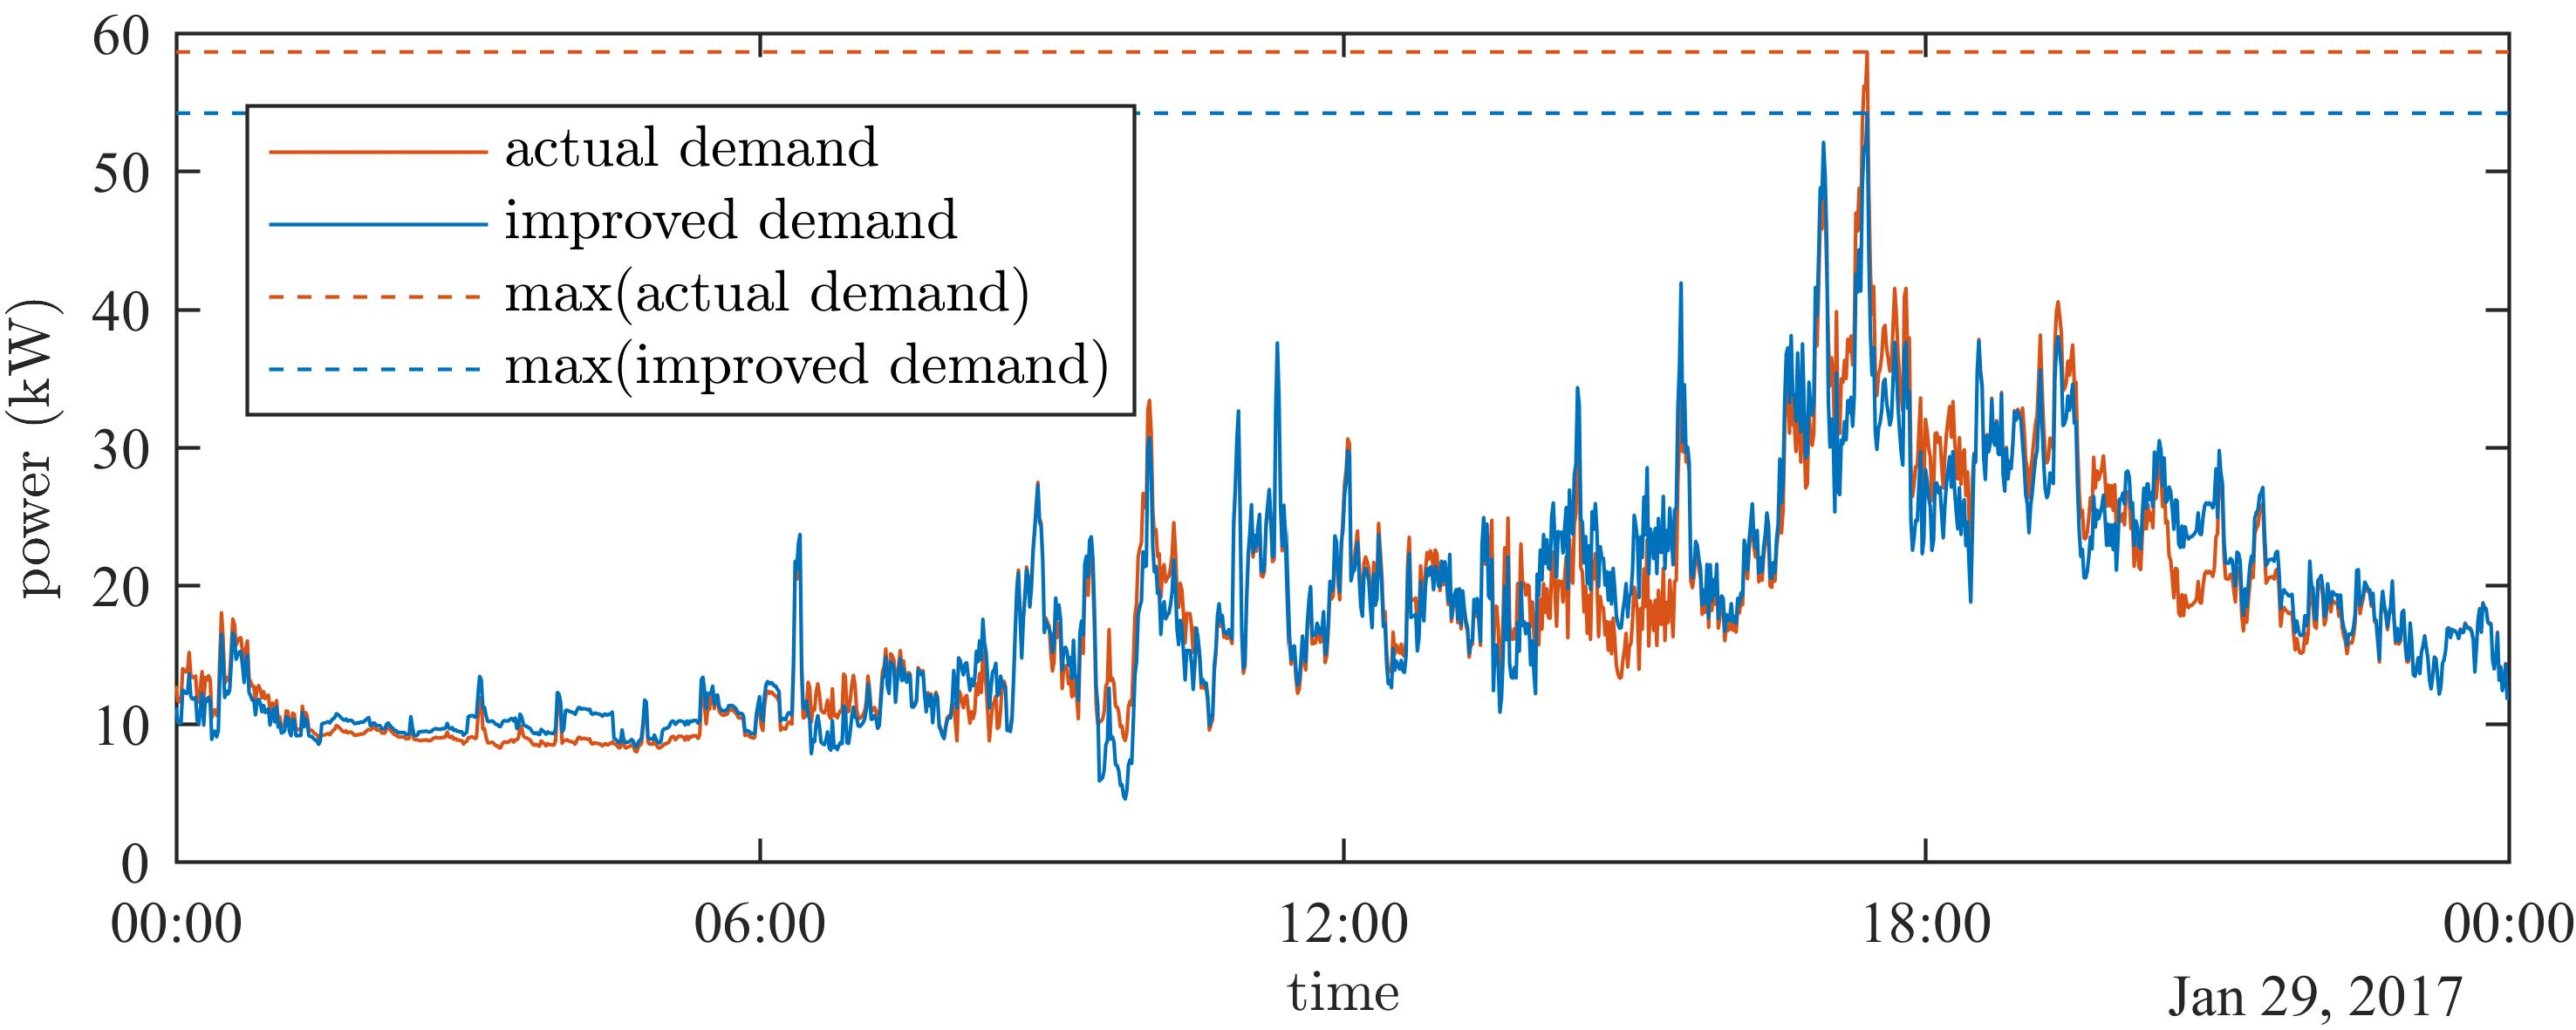
\includegraphics{_chapter2/fig/day-actual}
		\label{ch2:subfig:actual-forecasted}
	}
	\caption{An example of applying a half-hourly ESMU schedule to the half-hourly substation load (Subfig. \ref{ch2:subfig:day-forecasted}) and the actual, sub-half-hourly daily load, measured at the substation (Subfig. \ref{ch2:subfig:actual-forecasted}).}
	\label{ch2:fig:cost-sample}
\end{figure}

As repetitively mentioned, the ESMU operation that results from this scheduling mechanism is at half-hourly resolution and has therefore limited impact on sub-half-hourly load variation.
To visualise this limitation, a singe day's ESMU schedule was generated from its corresponding forecast as defined in Equation \ref{ch2:equ:cost-minimisation}, and plotted in Figure \ref{ch2:fig:cost-sample}.
In this simple comparison, the noticeable discrepancy between the half-hourly ESMU schedule and the actual, sub-half-hourly demand can be observed.
Furthermore, noticeable disparity in peak duration, magnitude and volatility can be noted.
This discrepancy and disparity emphasise the incompatibility issues between half-hourly ESMU schedules and the actual sub-half-hourly load.
As previously discussed, benefits of ESMU were intended to mitigate sub-half-hourly load volatility, yet this cannot be achieved when solely applying half-hourly ESMU schedules in an off-line manner.
Therefore, in the next section, the control strategy to add an on-line component is explained.




 

\section{Control of ESMU}
\label{ch2:sec:control-of-esmu}

\begin{figure}\centering
% Define some block styles
\tikzstyle{box} = [%
	draw,%
	rectangle,%
	%fill=green!20,%
	minimum height=3em,%
	minimum width=5em,%
]
\begin{tikzpicture}[node distance=2cm, shorten >= 1pt, >=stealth', auto, scale=0.8, transform shape]
	% Define nodes
    \path
    (0,0)
    node [box, minimum width=5cm, yshift=0mm](network) {Network}
    node [box, below of=network, yshift=0mm](battery) {Battery}
    node [box, fill=green!20, below left of=battery, yshift=-20mm, xshift=-10mm](pid_soc) {PID$_1$}
    node [box, fill=green!20, below right of=battery, yshift=-20mm, xshift=10mm](pid_p) {PID$_2$}
    node [box, fill=blue!20, below of=pid_soc, yshift=-15mm](schedule) {Schedule}
    node [box, fill=green!20, below of=pid_p, yshift=-15mm](mpc) {MPC};
	% Draw lines
	\draw [->] (battery) to (network);
	\draw [->, bend right] (pid_soc) to node[left, pos=0.4, xshift=-1mm] {$p_{1}(t+\Delta t)$} (battery);
	\draw [->, bend left] (pid_p) to node[right, pos=0.4, xshift=1mm] {$p_{2}(t+\Delta t)$} (battery);
	\draw [->] (battery.180) to [out=180, in=120] node[left, pos=0.2, xshift=-5mm] {$SOC^*(t)$} (pid_soc.180|-pid_soc.90);
	\draw [->] (network.0) to [out=340, in=60] node[left, pos=0.4] {$p_\text{net}(t)$} (pid_p.0|-pid_p.90);
	\draw [->] (schedule) to node[pos=0.25] {$SOC(t)$} (pid_soc);
	\draw [->] (mpc) to node[pos=0.25] {$\hat{p}_\text{net}(t+\Delta t)$} (pid_p);
	\draw [->, bend left] (network.0) to [out=80, in=100] node[right, pos=0.1, xshift=2mm, yshift=1mm] {$p_\text{net}(t)$} (mpc.0);
	
	\draw (-5, -6.75) node [right] {Controller};
	
	\draw [dashed] (-5, -3.5) -- (5, -3.5) -- (5, -6.5) -- (-5, -6.5) -- (-5, -3.5);
%	\draw [->, bend right] (schedule.180) to (controller.90);
%	\draw [->] (network) to (mpc);
%	\draw [->] (mpc) to (controller);
%	\draw [->] (controller) to (battery);
%	\draw [->] (battery) to (network);
\end{tikzpicture}%


\caption{Dynamic controller breakdown as previously shown in Figure \ref{ch2:subfig:proposed-dynamic-control-system}.}
\label{ch2:fig:system-controller}
\end{figure}


\hl{This section explains the dynamic control (i.e. the controller block as shown in Figure~}\ref{ch2:subfig:proposed-dynamic-control-system}\hl{) in the shape of an MPC, containing the two PID compensators to adjust operation around the predetermined ESMU schedule.}
The first PID compensator is fed by the ESMU schedule and the other is fed by the predictor load estimations.
After the control system is detailed in this section the auto-regressive models which were used during the course of this research are also explained.

\subsection{Dynamic control}

The content of the dynamic control procedure is shown in Figure~\ref{ch2:fig:system-controller}.
Here two reference signals are used as inputs to the dynamic control.
The first reference signal is the SOC profile derived from the ESMU scheduled, $SOC(t)$, and the second is an estimated future network power, $\hat{p}_\text{net}(t+\Delta t)$.
These two inputs are fed into compensator PID$_1$ and compensator PID$_2$, respectively.
The output of each compensator is a corrective battery power component that, when summed, yields the next ESMU power (i.e. $p_1(t+\Delta t)$ and $p_2(t+\Delta t)$) which is applied to the ESMU model.
Each PID compensator also receives a feedback signal to compute the internal error states.
More specifically, PID$_1$ receives the most recent SOC value that is obtained from the ESMU model, $SOC^*(t)$, and PID$_2$ receives the network's most recent power demand, $p_\text{net}(t)$ (for example through measurements by substation monitoring).

\nomenclature[J]{$p_\text{net}(t)$}{Most recent network demand at sample $t$, where $\textbf{p}_{net} = (p_\text{net}(t))$ and $p_\text{net}(t) \in \mathbb{R}$}
\nomenclature[J]{$SOC^*(t)$}{Battery's state of charge at sample $t$, where $SOC^*(t) \in [0, 1]$}
\nomenclature[J]{$E_\text{SOC}(t)$}{Error in state of charge at sample $t$, where $E_\text{SOC}(t) \in \mathbb{R}$}
\nomenclature[J]{$E_{p}(t)$}{Difference between current and predicting network power at sample $t$, where $E_{p}(t) \in \mathbb{R}$}
\nomenclature[J]{$\hat{p}_\text{net}(t+\Delta t)$}{Predicted next network power at sample $t$}
\nomenclature[J]{$\boldsymbol{\alpha}$}{PID weight vector for SOC compensator PID$_1$, where $\boldsymbol{\alpha} = \{\alpha_P, \alpha_I, \alpha_D\}$ and $\boldsymbol{\alpha} \in \mathbb{R}^3$}
\nomenclature[J]{$\boldsymbol{\beta}$}{PID weight vector for predictor compensator PID$_2$, where $\boldsymbol{\beta} = \{\beta_P, \beta_I, \beta_D\}$ and $\boldsymbol{\beta} \in \mathbb{R}^3$}
\nomenclature[J]{$\textbf{a}$}{Weight vector for compensator input regression of the AR model, where $\textbf{a} = \mathbb{R}^{N}$}
\nomenclature[J]{$\textbf{b}$}{Weight vector for compensator output regression of the AR model, where $\textbf{b} = \mathbb{R}^{N}$}
\nomenclature[J]{$N$}{Number of regressors of the AR model, where $N \in \mathbb{Z}_{>0}$}
\nomenclature[J]{$p_1(t)$}{Corrective ESMU power components from PID$_1$, where $p_1(t) \in \mathbb{R}$}
\nomenclature[J]{$p_2(t)$}{Corrective ESMU power components from PID$_2$, where $p_2(t) \in \mathbb{R}$}
\nomenclature[J]{$SOC_{tol}$}{SOC tolerance, i.e. maximum deviation from the prescheduled SOC profile, where $SOC_{tol} \in [0, 0.5]$}

Inside the PID$_1$ component a SOC error term, $E_\text{SOC}(t)$, is computed.
This term is the difference between the scheduled SOC profile, $SOC(t)$, and the actual (or simulated) SOC values, $SOC^*(t)$.
The following equation captures this error term.

\begin{equation}
	E_{SOC}(t) := SOC^*(t) - SOC(t)
	\label{ch2:equ:soc-error}
\end{equation}

Applying a standard and linearly weighted dynamic gain vector, $\boldsymbol{\alpha}$, to the SOC error allows the calculation of a corrective ESMU power component dynamically.
Here $\boldsymbol{\alpha} = \{\alpha_P, \alpha_I, \alpha_D\}$ and the components are the P, I and D weights, respectively.
How to determine the values of $\boldsymbol{\alpha}$ is explained later in this section.
This corrective power is denoted as $p_1(t+\Delta t)$, and is defined as follows:

\begin{equation}
\begin{split}
	p_1(t+\Delta t) &:= \alpha_P E_{SOC}(t)\\
	&+ \alpha_I \sum_{i=0}^\infty E_{SOC}(t-i\Delta t)\\
	&+ \alpha_D \frac{E_{SOC}(t)-E_{SOC}(t-\Delta t)}{\Delta t}
\end{split}
\label{ch2:equ:corrective-component-soc}
\end{equation}

Here the integral component removes steady-state error and the instantaneous error differential prevents overshooting.
All in all, this compensator uses present and past values to issue a corrective future ESMU instruction.
Compensator PID$_2$ on the other hand uses values from the present, past and future in order to minimise the power transient and load peaks.

\begin{figure}[htb]\centering
% Define some block styles
\tikzstyle{box} = [%
	draw,%
	rectangle,%
	%fill=green!20,%
	minimum height=3em,%
	minimum width=5em,%
]
\tikzstyle{sample} = [draw, circle, fill, scale=0.4]
\tikzstyle{estimate} = [draw, circle, solid, fill=white, scale=0.4]
\begin{tikzpicture}[node distance=2cm, shorten >= 1pt, >=stealth', auto, scale=0.9, transform shape]
	% Draw axis and labels
	\draw [<->] (0, 6) -- (0, 0) -- (12, 0);
	\draw (12, 0) node [anchor=north east] {Time};
	\draw (0, 3) node [anchor=south, rotate=90] {Power};
	% Add axis ticks
	\foreach[count=\i, evaluate=\i as \l using int(\i-1)] \t in {1,4,...,10}
	{
		\draw (\t,0.1) -- (\t,-0.1);
		\ifthenelse{\l=0}
		{\draw (\t,-0.1) node[anchor=north] {$t$}}
		{
			\ifthenelse{\l=1}
			{\draw (\t,-0.1) node[anchor=north] {$t+\tau$}}
			{\draw (\t,-0.1) node[anchor=north] {$t+\l\tau$}};
		};
	}
	% Draw main power curve
	\draw [thick]
	(0.5, 2.1) to
	(1, 2) node[sample](sam_0) {} to
	(4, 4) node[sample](sam_1) {} to
	(7, 3.5) node[sample](sam_2) {} to
	(10, 2) node[sample](sam_3) {} to
	(11, 1.8);
	
	% Add power sample forward projection
	\draw [dashed] (1, 2) -- (4.6, 2);
	\draw [dashed] (4, 4) -- (7.5, 4);
	\draw [dashed] (7, 3.5) -- (10.5, 3.5);
	\draw [dashed] (10, 2) -- (10.5, 2);
	
	% Plot estimates
	\draw [dotted] (1, 2) to
	(4, 3.7) node[estimate](est_1) {} to
	(7, 3.8) node[estimate](est_2) {} to
	(10,1.7) node[estimate](est_3) {};
	
	% Label the power samples
	\draw [->] (1, 5) node[anchor=south] {$p(t)$} to [out=-135,in=135] (sam_0);
	\draw [->] (4, 5) node[anchor=south] {$p(t+\tau)$} to [out=-135,in=135] (sam_1);
	\draw [->] (7, 5) node[anchor=south] {$p(t+2\tau)$} to [out=-135,in=135] (sam_2);
	\draw [->] (10, 5) node[anchor=south] {$p(t+3\tau)$} to [out=-135,in=135] (sam_3);
	
	% Label the estimates
	\draw [->] (4, 0.75) node[anchor=north] {$\hat{p}(t+\tau)$} to [in=-45] (est_1);
	\draw [->] (7, 0.75) node[anchor=north] {$\hat{p}(t+2\tau)$} to [in=-45] (est_2);
	\draw [->] (10, 0.75) node[anchor=north] {$\hat{p}(t+3\tau)$} to [in=-45] (est_3);
	
	% Label the forward power transients
	\draw [decorate,decoration={brace,amplitude=3pt,mirror,raise=4pt},yshift=0pt,xshift=5mm]
	(4, 2) -- (4, 4) node [anchor=west,black,midway,xshift=2mm] {$\epsilon_p(t)$};
	\draw [decorate,decoration={brace,amplitude=3pt,mirror,raise=4pt},yshift=0pt,xshift=3mm]
	(7, 3.5) -- (7, 4) node [anchor=west,black,midway,xshift=2mm] {$\epsilon_p(t+\tau)$};
	\draw [decorate,decoration={brace,amplitude=3pt,mirror,raise=4pt},yshift=0pt,xshift=3mm]
	(10, 2) -- (10, 3.5) node [anchor=west,black,midway,xshift=2mm] {$\epsilon_p(t+2\tau)$};
	
\end{tikzpicture}
%	\draw [solid] (12, 6) -- (12, 4.75) -- (10.5, 4.75) -- (10.5, 6) -- (12, 6);
%	\draw (10, 6) node[sample, yshift=-10mm, xshift=25mm](legend_sample) {};
%	\draw node[right of=legend_sample, xshift=-15mm] {$p$};
%	\draw (10, 6) node[estimate, yshift=-20mm, xshift=25mm](legend_estimate) {};
%	\draw node[right of=legend_estimate, xshift=-15mm] {$\hat{p}$};
\caption{Underlying time-series based compensation strategy for compensator PID$_2$. Here, $p_{network}$ and $\hat{p}_{network}$ are abbreviated to $p$ and $\hat{p}$, respectively.}
\label{ch2:fig:power-transient-minimisation}
\end{figure}


Figure~\ref{ch2:fig:power-transient-minimisation} summarises the time series computations for each power sample at times $t$, $t+\Delta t$, etc.
Ideally, PID$_2$ uses present power readings, $p_\text{net}(t)$, and a power value of the immediate future, i.e. $p_\text{net}(t+\Delta t)$, to compute a power error signal, which is to be reduced to a smallest possible value.
This error signal is defined as:

\begin{equation}
	E_p(t) := p_\text{net}(t+\Delta t) - p_\text{net}(t)
	\label{ch2:equ:power-error-signal}
\end{equation}

However, since the future network power is unknown an ``estimated next power'', $\hat{p}_\text{net}(t+\Delta t)$, is used instead.
This value is the PID$_2$'s input from the predictor and results in an ``estimated power error signal'':

\begin{equation}
	\hat{E}_{p}(t) = \hat{p}_{net}(t+\tau) - p_{net}(t)
	\label{ch2:equ:power-error-estimate}
\end{equation}

Similarly to PID$_1$, PID$_2$ produces a corrective ESMU power component, $p_2(t)$, that smoothens the resulting power profile.
This corrective ESMU power is also computed using a standard linear weighted dynamic vector $\boldsymbol{\beta}$, with $\boldsymbol{\beta} = \{\beta_P, \beta_I, \beta_D\}$, being the P, I and D weight, respectively:

\begin{equation}
\begin{split}
	p_2(t+\tau) &:= \beta_P E_{p}(t)\\
	&+ \beta_I \sum_{i=0}^\infty E_{p}(t-i\tau)\\
	&+ \beta_D \frac{E_{p}(t)-E_{p}(t-\tau)}{\tau}
\end{split}
\label{ch2:equ:corrective-component-power}
\end{equation}

Similar to $\boldsymbol{\alpha}$ how to determine the values of $\boldsymbol{\beta}$ is explained later in this section.
Finally, the ``next ESMU power'' can be deduced by adding the two corrective ESMU power components, as shown in the equation below.

\begin{equation}
	p(t+\Delta t) = p_1(t+\Delta t) + p_2(t+\Delta t)
	\label{ch2:equ:next-battery-power}
\end{equation}

Both PID compensators do however depend on correctly chosen weights for $\boldsymbol{\alpha}$ and $\boldsymbol{\beta}$.
Therefore they need to be tuned prior to executing the dynamic control.
For this work a minimisation problem was formulated that is based on a cost function, $\zeta^*(\boldsymbol{\alpha}, \boldsymbol{\beta})$, to deduce the two weight vectors as follows:

\begin{equation}
	\min_{\alpha,\beta} \zeta^*(\alpha, \beta) \text{ s.t. }
	\begin{cases}
		SOC(t) - SOC_{tol} \leq 0\\
		-SOC(t) \leq 0\\
		SOC(t) - 1 \leq 0
	\end{cases}
	\forall t
	\label{ch2:equ:cost-weights}
\end{equation}

Here, $\zeta^*(\boldsymbol{\alpha}, \boldsymbol{\beta})$ is defined as:

\begin{equation}
\begin{split}
	\zeta^*(\boldsymbol{\alpha}, \boldsymbol{\beta}) := \max_t(\textbf{p}_{net} + \textbf{p})\\
	\text{ where } \textbf{p}_{net} = (p_\text{net}(t)) \text{ and } \textbf{p} = (p(t))
\end{split}
\label{ch2:equ:dynamic-cost}
\end{equation}

In Equation~\ref{ch2:equ:cost-weights} and Equation~\ref{ch2:equ:dynamic-cost}, $\zeta^*(\boldsymbol{\alpha}, \boldsymbol{\beta})$ represents the sub-half-hourly peak load during a day when ESMU schedules are adjusted with the corresponding $\boldsymbol{\alpha}$ and $\boldsymbol{\beta}$ weights.
Also, the same SOC tolerance that was used to generate the SOC schedule (i.e. $SOC_{tol}$) is included to prevent the solution from deviating off the prescheduled SOC profile.
To generalise this solution for all load cases this minimisation problem was formulated to solve multiple daily load profiles in order to find ideal values for $\boldsymbol{\alpha}$ and $\boldsymbol{\beta}$.
\hl{The system of two PID compensators for discrete time is unconventional and it is worth considering different types of control or compensator.
However, with the above-explained approach and for the data used as part of this research, the computed set of $\boldsymbol{\alpha}$ and $\boldsymbol{\beta}$ weights resulted a convergent and stable solutions.
In this context, convergent means that the $SOC^*(t)$ values tend towards the $SOC(t)$ values, and stable means that the $SOC^*(t)$ values never clipped at zero or one.
The details concerning these case studies themselves are however outlined in Section~}\ref{ch2:sec:case-studies}\hl{.}

\subsection{Model predictive control}

As explained in the literature review in Chapter~\ref{ch-literature}, Model Predictive Control (MPC) is favoured over Set-Point Control (SPC), since it takes into account time-series to produce a behaviour.
With this knowledge, MPC can be used to not only react to recent changes but also to counteract foreseen trends.
Different approaches exist to obtain these foreseen trends and these approaches highly vary in accuracy, computational burden and robustness.
Equally, the characteristics of underlying data which is used to train these models impacts their performances.
For the presented work in this chapter, an efficient and robust approach is required since potential ESMU deployment with SSEN demands these functional requirements.
Prediction accuracy on the other hand is an optional requirement which becomes important only when the predicting model can issue predictions in real-time and does (for the predicting horizon) remain stationary and bounded.

The simplest form of producing a prediction is to assume that the currently observed trending load will also occur in the future.
This kind of prediction does however not take into account demand dynamics.
%Instead, it uses the mean power which is explained as follows:
%
%\begin{equation}
	\hat{p}(t+\Delta t) = \frac{1}{N}\sum_{i=0}^{N-1}p(t-i\Delta t)
	\label{ch2:equ:simple-prediction}
\end{equation}
%
%Here, the estimated next power, $\hat{p}(t+\Delta t)$, is derived as the average past powers, $p(t)$, over an averaging horizon, $N$.
An AR model on the other hand uses a series of past observations and their individual contribution to predict the next power.
But the further into the future these predictions are made the less accurate they become.
This accuracy loss is however circumvented since the hybrid system was designed to only apply corrections based on load predictions of the immediate future (i.e. next sample time at $t+\Delta t$ and not $t+2\Delta t$ or similar).
This simplification also reduces computational burden and guarantees real-time operation especially when choosing the simplest dynamic model (i.e. an Auto-Regressive (AR) model instead of deep artificial neural networks).
Since external forces can and often do impact the behaviour of the model, the AR model is treated as an exogenous model with a time-series of input powers, $\textbf{p} = (p(t))$, a time-series of predicted ``next powers'', $\hat{\textbf{p}} = (\hat{p}(t))$, and an internal delay function $t-\Delta t$.

\begin{figure}\centering
% Define some block styles
\tikzstyle{box} = [%
	draw,%
	rectangle,%
	%fill=green!20,%
	minimum height=2em,%
	minimum width=2em,%
]
\begin{tikzpicture}[node distance=2cm, shorten >= 1pt, >=stealth', auto, scale=0.9, transform shape]
	\pgfmathsetmacro\N{4}

	% Draw input nodes
    \draw
    (0, 0) node [](input) {$p(t)$}
    (1, 0) node [](input_1) {};
    % Draw output nodes
    \draw
    (6.5, 0) node [](output) {$\hat{p}(t+\Delta t)$}
    (5, 0) node [](output_1) {};
    % Draw main adder node
    \draw (3, 0) node [circle, draw](adder_main) {+};
    % Link input, adder and output
    \draw [->] (input) to (adder_main);
    \draw [->] (adder_main) to (output);
    % Draw AR model nodes
    \foreach[count=\i, evaluate=\i as \l using int(\i*2)] \n in {1,2,...,\N}
	{
		\ifthenelse{\n<\N}
		{
	    	\draw (1, 1-\l) node [box](z_a\n) {$z^{-1}$};
	    	\draw (1, -\l) node [](half_a\n) {};
	    	\draw (1.8, -\l) node [box](a\n) {$a_\n$};
	    	
	    	\draw (5, 1-\l) node [box](z_b\n) {$z^{-1}$};
	    	\draw (5, -\l) node [](half_b\n) {};
	    	\draw (4.2, -\l) node [box](b\n) {$b_\n$};
	    	
	    	\draw (3, -\l) node [circle, draw](adder_\n) {+};
    	}{
	    	\draw (1, 1.95-\l) node [](z_a\n) {};
	    	\draw (5, 1.95-\l) node [](z_b\n) {};
    	}
    	\ifthenelse{\n=1}
    	{
    		\draw [->] (input_1.center) to (z_a\n);
    		\draw [->] (output_1.center) to (z_b\n);
    		\draw [->] (adder_\n) to (adder_main);
    	}{
    		\pgfmathtruncatemacro{\dn}{\n-1};
    		\pgfmathtruncatemacro{\dnn}{\n-2};
    		\ifthenelse{\n<\N}
			{
				\ifthenelse{\dn=1}
				{
					\draw [->] (z_a\dn) to node[left]{$p(t-\Delta t)$} (z_a\n);
				}{
					\draw [->] (z_a\dn) to node[left]{$p(t-\dn\Delta t)$} (z_a\n);
				}
				\ifthenelse{\dnn=0}
				{
					\draw [->] (z_b\dn) to node[right]{$\hat{p}(t)$} (z_b\n);
				}{
					\ifthenelse{\dnn=1}
					{
						\draw [->] (z_b\dn) to node[right]{$\hat{p}(t-\Delta t)$} (z_b\n);
					}{
						\draw [->] (z_b\dn) to node[right]{$\hat{p}(t-\dnn\Delta t)$} (z_b\n);
					}
				}
				\draw [->] (adder_\n) to (adder_\dn);
			}{
				\draw [-] (z_a\dn) to node[left]{$p(t-\dn\Delta t)$} (z_a\n.center);
				\draw [-] (z_b\dn) to node[right]{$\hat{p}(t-\dnn\Delta t)$} (z_b\n.center);
			}
    		\draw [->] (half_a\dn.center) to (a\dn);
    		\draw [->] (a\dn) to (adder_\dn);
    		\draw [->] (half_b\dn.center) to (b\dn);
    		\draw [->] (b\dn) to (adder_\dn);
    	}
    }

\end{tikzpicture}
\caption{Exogenous auto-regressive model that is used for model predictive control. Here, $z^{-1}$ indicates the time delay by one sample period, i.e. $\Delta t$.}
\label{ch2:fig:mpc-arx}
\end{figure}


Figure~\ref{ch2:fig:mpc-arx} graphically captures the standard AR model's function tree which is equivalently represented mathematically in the following equation:

\begin{equation}
\begin{split}
	\hat{p}(t+\Delta t) &= p(t) + \sum_{i=1}^{N} a_i p(t-i\Delta t)\\
	&+ \sum_{i=1}^{N} b_i \hat{p}(t-(i-1)\Delta t)
\end{split}
\label{ch2:equ:mpc-arx}
\end{equation}

Values of the two weight vectors $\textbf{a}$ and $\textbf{b}$, where $\textbf{a} = (a_i)$ and $\textbf{b} = (b_i)$, are determined during runtime using the standard adaptive least squares algorithm, i.e.:

\begin{equation}
	\min_{\textbf{a}, \textbf{b}} \left(p(t) - \hat{p}(t)\right)^2
\label{ch2:equ:least-squares-1}
\end{equation}
Or:
\begin{equation}
	\min_{\textbf{a}, \textbf{b}} \left(p(t) - p(t - \Delta t) + \sum_{i=2}^{N} a_i p(t-i\Delta t) + \sum_{i=2}^{N} b_i \hat{p}(t-(i-1)\Delta t)\right)^2
\label{ch2:equ:least-squares-2}
\end{equation}


Therefore, the proposed algorithm adjusts $\textbf{a}$ and $\textbf{b}$ to minimise the prediction error at each time-step.
Beside finding optimised values for $\textbf{a}$ and $\textbf{b}$, the model's number of regressors, $N$, is also expected to impact the model's performance ($N$ is also referred to as the ``model length'').
The example in Figure~\ref{ch2:fig:mpc-arx} represents a symmetric model where $N=3$.
This short length however is most likely insufficient in predicting $p(t+\Delta t)$ which is why several models of increasing lengths are assessed and compared in the results section of this chapter.
From this comparison the impact of $N$ on the models' resulting values of $\hat{p}(t+\Delta t)$ and correspondingly on the performance of the dynamic controller can be determined and discussed.
Details about the cases for different model length are presented in the case studies in Section~\ref{ch2:sec:case-studies}.


\section{Case studies}
\label{ch2:sec:case-studies}

Two cases are defined that the performance of the proposed dynamic control is compared against: case \textbf{O} and case \textbf{B}.
More specifically, case \textbf{O}, original case, is the scenario where no BESS operation takes place.
Traditional off-line BESS operation that only uses predetermined half-hourly BESS schedules is referred to as the benchmark case, or case \textbf{B}.
All remaining cases, which are explained below, are capture different versions of the dynamic control.

In addition to the two comparison cases, three more different case studies are defined: cases \textbf{I}, \textbf{II} and \textbf{III}.
This group of three case studies evaluates the impact of the proposed dynamic control when subjected to realistic (i.e. imperfect) half-hourly load forecasts.
In each of the three cases, a different mechanisms is used to predict the power volatility.
More specifically:
\begin{itemize}
	\item case \textbf{I} implements the simplest prediction mechanism, i.e. it is assumed that the current power measurements repeats,
	\item case \textbf{II} uses the aforementioned MPC, and performance of different AR model lengths is compared, and
	\item case \textbf{III},the third and final case, represents an ideal scenario where perfect foresight is assumed and the exact next load can be estimated.
\end{itemize}
For clarity, all three cases, numbered \textbf{I} to \textbf{III}, are summarised and tabulated in Table \ref{ch2:tab:cases}.

\begin{table}[htb]\centering
	\begin{tabular}{r | c c}
		& real forecast & ideal forecast\\
		\hline
		repeated power estimation & \textbf{I} & \textbf{IV}\\
		MPC power estimation & \textbf{II} & \textbf{V}\\
		perfect power foresight & \textbf{III} & \textbf{VI}\\
	\end{tabular}
	\caption{Six cases and their dynamic control input assumptions}
	\label{ch2:tab:cases}	
\end{table}

Results from all BESS cases (\textbf{B}, \textbf{I}, \textbf{II} and \textbf{III}) are first compared against the original, i.e. uncompensated, network load case (\textbf{O}).
Here, by using a sample day, the assessment of load profile improvements are made clear.
Once it is clear how each day's peak is reduced by the algorithm, the daily peak reduction capability from all cases' results are compared.
Rather than assessing the underlying load profile from a time-series perspective, only focus is put on any further peak load reductions.
However, the number of days may make it difficult to spot trends and improvements in the data.
Therefore, from the daily peak reduction results, a Probability Density Function (PDF) is derived, which is based on kernel density estimation.
The PDF shows the stochastic improvement of each case type in comparison to the original case, i.e. case \textbf{O}.


\section{Results and Discussion}
\label{ch1:sec:results-and-discussion}


\section{Conclusion}
\label{ch2:sec:conclusion}

%%%%%%%%%%%%%%%%%%%%%%%%



\section*{References}

\bibliography{../Bibliography/library}

\end{document}